\documentclass{article}
\usepackage{graphicx} % Required for inserting images\
\usepackage{hyperref}
\usepackage{xcolor}
\usepackage{amsmath,amssymb}
\usepackage{natbib}
\usepackage{booktabs}
\usepackage{float}

% sets
\newcommand{\mA}{\mathcal{A}}
\newcommand{\mD}{\mathcal{D}}
\newcommand{\mE}{\mathcal{E}}
\newcommand{\mN}{\mathcal{N}}
\newcommand{\mP}{\mathcal{P}}
\newcommand{\mV}{\mathcal{V}}

% vectors
\newcommand{\bw}{\boldsymbol{w}}
\newcommand{\bx}{\boldsymbol{x}}
\newcommand{\bz}{\boldsymbol{z}}


% Our macros
\newcommand{\margarida}[1]{\colorbox{teal}{\color{white}   \textsf{\textbf{Margarida}}} \textcolor{teal}{#1}}

\title{Decision focused learning for KEPs}

\date{March 2026}

\begin{document}

\maketitle

\section{Logistics}

Please register as a research intern in CIRRELT so that you can receive information on their activities and because this will be useful to have access to the computing grid: 
\href{https://www.cirrelt.ca/default.aspx?PAGE=INSCRIPTION}{Link for registration}

\section{Problem description}
In Section~\ref{subsec:setup}, we describe the typical information available before running a kidney exchange. Section~\ref{subsec:optimizationtask} provides an overview on what is a run of the kidney exchange, i.e., the optimization problem that is solved as all as relevant references of implemented KEPs. Section~\ref{subsec:predictiontask} discusses the predictions/estimations that are relevant when performing the optimization task of Section~\ref{subsec:optimizationtask}.

\subsection{Setup}\label{subsec:setup}
We are given a graph $G=(\mV,\mA)$ where $\mV$ consists of two disjoint sets:
\begin{itemize}
    \item $\mP$, the set of (incompatible) patient-donor pairs;
    \item $\mN$, the set of non-directed donors, also called \emph{altruistic donors}\footnote{This term has been less and less used because, in all fairness, the donors in $\mP$ are also involved in an altruistic act.} as they register in the KEP pool without a corresponding donor.
\end{itemize}
An arc $(v,u) \in \mA$ means that the donor of $v$ is compatible with the patient of $u$.

For each $v \in \mV$, we suppose to have a function $g(v): \mV \rightarrow \mathbb{S}^n$ which provides the covariates (vertex features) of the vertices, e.g., $g(v)$ returns the blood-type of the patient and donor associated to vertex $v$\footnote{If $v \in \mN$, then the donor's features are 0 (or NA?).}, patient cPRA (Calculated Panel Reactive Antibody), HLA antigens, time in dialysis, age, to name a few \margarida{We can check in the literature which features seem relevant for determining successful transplant}. 

\subsection{Optimization task: Exchange plan}\label{subsec:optimizationtask}
In kidney exchange systems, we seek to find in $G$ disjoint sets of
\begin{itemize}
    \item \emph{cycles}: a cycle in $G$ must involve only vertices in $\mP$ and its length (i.e., number of contained vertices) should be at most $L$\footnote{Grafts associated with a cycle must be performed simultaneous and thus, due to logistic restrictions, it is undesirable to have large cycles. This motivates real-world implemented KEPs to have a predefined $L$. Moreover, if something goes wrong in a cycle (e.g., a donor drops-out), it is better to have small cycles because less patients are affected.}. In most KEPs, $L$ is 3 but, for example in Canada, it can go up to 5. If $L=2$ or unbounded, the optimization can be performed in polynomial time. Otherwise, for $L>2$ and bounded, the problem is NP-hard.
    \item \emph{chains}:  a chain in $G$ is initiated by a vertex in $\mN$ and then, it consists of vertices in $\mP$. The last patient-donor pair (vertex) in the chain donates to the next KEP run or to the waiting list of deceased donors. In many programs the maximum length of a chain can be fixed; however, contrary to cycles, grafts associated with a chain do not need to be done simultaneously because there is never the danger of a donor of a vertex $\mP$ having donate a kidney and now its patient being unable to receive one. 
\end{itemize}
A \emph{kidney exchange plan} for a given $G$ is thus a set of disjoint cycles and chains. The aim is to select a kidney exchange plan that optimizes the patient benefit and that is fair. In practice, the primary objective is typically the number of transplants. There are programs that implement an hierarchical optimization (starting by maximizing the number of transplants) and others that use a weighted objective. See \cite{biro2019building, biro2021modelling} describing the optimization of KEPs in Europe, \cite{carvalho2023penalties} which describes Canada's score system (table 3.1 of the long version of the paper) to build a weighted objective, and \cite{delorme2024new} who discuss hierarchical optimization in KEPs.

Let $\mE$ be the set of feasible exchanges (i.e., cycles and chains in $G$ respecting length limitations). In KEPs using weighted objectives, we aim to solve the following optimization
\begin{align}
    & \max_{\bz} & \sum_{e \in \mE} w_e z_e \\
    & s.t. & \sum_{e \in \mE: v \in e} z_e \leq 1 &\quad  \forall v \in \mV \textrm{ (each donor donates once)}\\
    & & \bz \in \{0,1\}^{\mE},
\end{align}
where $w_e$ represents the weight of exchange $e$ (e.g., the benefit for the patients involved in exchange $e$, the length of the exchange which is the number of patients receiving a kidney). Of course, constructing $\mE$ is not practical for large size $G$ ($|\mV|>200$), so it is relevant to consider other formulations (see Section 3 the survey by~\cite{barkel2025operational}); for sake of simplicity, for the problem description, we keep this simple formulation.

\subsection{Prediction task: benefit of an exchange} \label{subsec:predictiontask}
Suppose we have data from previous KEP runs:
$$\mD=\{ (\bx^i, \bw^i) \}_{i=1}^N,$$
where $\bx^i=(G^i=(\mV^i,\mA^i), \{g(v)\}_{v \in \mV^i}) $ are our covariates (graph plus vertices features) and $\bw^i=\{ w^i_e \}_{e \in \mE^i \wedge z^i_e=1}$ is the benefit of the performed exchanges. This benefit $w_e^i$ can represent \margarida{This list is not exhaustive and we should go over the literature on KEPs under uncertainty to extract what are the most common predictions used.}
\begin{itemize}
    \item the probability that the exchange goes through, i.e., no involved donor drops-out and no involved patient has their health-status deteriorated such that graft is not possible;
    \item the quality-adjusted life year (QALY)~\citep{glorie2022health};
    \item a combination of the aforementioned points (weighted objective);
    \item patient utility associated with a graft from a specific donor;
    \item expected number of years added to the patient’s lifespan~\citep{krikov2007predicting}.
\end{itemize}


In this way, our optimization becomes
\begin{align}
    & \max_{\bz} & \mathbb{E}_{\bw | \bx }\left[\sum_{e \in \mE} w_e z_e \right] &= \sum_{e \in \mE} \mathbb{E}_{\bw | \bx }\left[w_e \right] z_e\\
    & s.t. & \sum_{e \in \mE: v \in e} z_e \leq 1 &\quad  \forall v \in \mV \textrm{ (each donor donates once)}\\
    & & \bz \in \{0,1\}^{\mE}.
\end{align}
The literature on KEPs has consider cases where the distribution of $\bw$ is known~\citep{alvelos2019maximizing} or where a worst-case analysis (robust optimization) is done~\citep{carvalho2021robust,blom2024cutting}. In this work, we assume to have only access to $\mD$ and not the distribution of $\bw | \bx$.

\margarida{
See references that consider prediction tasks for living donation so that we can have an idea of how to generate covariates and the ground truth for $\bw$. For example, check ~\cite{massie2016risk,luck2017deep,monteiro2019reinforcement}.
}


\subsubsection{Constraints}
In the optimization above, the uncertainty is in the objective. Previous literature in DFL has looked to this case where the prediction model impacts the objective function. The case where the uncertainty is in the constraints has had less (none?) attention. There are some works in KEP that propose additional constraints for KEPs, namely, related with fairness (e.g., being sure that the distribution of patients blood-type follows the distribution in the population; it is undesirable to accumulate O-blood type patients). Hence, it might make sense to reflect on uncertainty in the constraints.



\section{Experiments}
\label{sec:experiments}
This section evaluates whether decision-focused learning improves final kidney exchange plans compared with a standard two-stage pipeline. We compare methods on synthetic KEP instances generated with donor/patient medical attributes and edge-level utilities, then assess both prediction quality and downstream optimization quality.

\subsection{Research questions}
Our experiments address the following questions:
\begin{itemize}
    \item Does end-to-end decision-focused learning produce better exchange plans than predict-then-optimize baselines?
    \item Does a graph-based predictor (GNN) outperform a non-graph baseline (MLP/Regression) on final optimization metrics?
    \item How large is the gap between learned models and an oracle that optimizes with ground-truth edge benefits?
\end{itemize}

\subsection{Data and Instance Construction}
\subsubsection{Synthetic KEP instance generation}
Synthetic instances follow the Saidman-style construction paradigm~\citep{saidman2006increasing}. Each instance is a directed compatibility graph with patient-donor pairs and altruistic donors, generated from prespecified demographic and immunological distributions. In addition, recipient ages are sampled uniformly in \([18,68]\), and edge-level compatibility scores are interpreted as utility values.

All generation settings used in our experiments are centralized in this subsection. Numeric parameters consistent with this setup are summarized in Table~\ref{tab:generation-params}. Non-numeric modeling choices are:
\begin{itemize}
    \item \textbf{Distribution matching}: enabled to reduce deviations between empirical and target marginal distributions.
    \item \textbf{Donor blood-type model}: a global donor blood-type distribution is used (rather than recipient-type-specific donor distributions).
    \item \textbf{Sensitization and compatibility bands}: cPRA and compatibility are sampled from fixed band-based rules.
\end{itemize}

\begin{table}[H]
\centering
\caption{Default numeric parameters for synthetic KEP generation.}
\label{tab:generation-params}
\begin{tabular}{|l|l|l|}
\hline
\textbf{Category} & \textbf{Parameter} & \textbf{Value} \\
\hline
Scale & Number of instances & 1000 \\
 & Patients per instance & 50 \\
 & NDD proportion & 0.05 \\
\hline
Patient blood type & \(P(O)\) & 0.4 \\
 & \(P(A)\) & 0.4 \\
 & \(P(B)\) & 0.1 \\
 & \(P(AB)\) (computed residual) & 0.1 \\
\hline
Donor blood type & \(P(O)\) & 0.4 \\
 & \(P(A)\) & 0.4 \\
 & \(P(B)\) & 0.1 \\
 & \(P(AB)\) (computed residual) & 0.1 \\
\hline
Donor count per pair & \(P(1)\) donor & 1.0 \\
 & \(P(2)\) donors & 0.0 \\
 & \(P(3)\) donors & 0.0 \\
 & \(P(4)\) donors (computed residual) & 0.0 \\
\hline
Base characteristics & Spousal donor probability & 0.0 \\
 & Female donor probability & 0.0 \\
 & Spousal PRA compatibility & 0.0 \\
\hline
Tuning & Iterations & 100 \\
 & Tuning sample size & 1000 \\
 & Error tolerance & 0.05 \\
\hline
Injected feature & Recipient age range & [18, 68] \\
\hline
\end{tabular}
\end{table}

\subsubsection{Graph processing and label definition}\label{subsubsec:graph-processing}
\paragraph{Graph Simplification.}
Raw donor-level instances are transformed into a unified exchange graph whose vertices are patient-donor pairs or altruistic donors. If multiple donor-level edges induce the same ordered pair of vertices $(i,j)$, only the edge with maximal utility is retained:
\[
u_{ij}^{\star}=\max_{e\in\mathcal{E}_{ij}} u_e .
\]

\paragraph{Node Features.}
Each node is represented by a 13-dimensional feature vector summarized in Table~\ref{tab:node-features}.

\begin{table}[t]
\centering
\caption{Node feature construction for pair and altruistic-donor vertices.}
\label{tab:node-features}
\begin{tabular}{@{}lp{0.72\linewidth}@{}}
\toprule
\textbf{Vertex type} & \textbf{Features} \\
\midrule
Patient-donor pair & Patient age; recipient cPRA; indicator for whether the patient has a blood-type-compatible donor; patient blood type encoded as a 4-dimensional one-hot vector $(O,A,B,AB)$; donor age; donor blood type encoded with the same 4-dimensional one-hot scheme; NDD indicator $=0$. \\
Altruistic donor & Patient-related entries are set to zero; donor age; donor blood type encoded as a 4-dimensional one-hot vector $(O,A,B,AB)$; NDD indicator $=1$. \\
\bottomrule
\end{tabular}
\end{table}
\paragraph{Graft Survival Time.}
Clinical proxy quantities are defined by the following mappings (with $a_d$ donor age, $c$ recipient cPRA, and edge utility $u$).
The first mapping computes a graft-survival-time proxy from donor age:
\[
T(a_d)=\max\{5,\ 25-0.3(a_d-20)\},
\]
where \(T(a_d)\) is a heuristic age-to-survival proxy introduced for synthetic label construction (not a clinically calibrated survival model).
\paragraph{Remark.}
This simplification is much narrower than the modeling perspective in~\citet{luck2017deep}. That work treats graft survival as a function of all available donor features, recipient features, donor-recipient couple characteristics, and transplant factors, rather than donor age alone; after feature filtering, their study uses 436 variables. The paper also highlights that donor age has a nonlinear effect, with donors younger than 21 associated with better graft survival. Accordingly, a formulation closer to that paper would be \(T(d,r)=f(a_d,x_d,x_r,x_{d,r},x_{\mathrm{tx}})\), whereas our current \(T(a_d)\) is only a minimal synthetic proxy.
\paragraph{Quality-Adjusted Life Years.}
The second mapping computes QALY by combining a utility-based quality factor with the survival-time proxy:
\[
\phi(u)=\frac{\sqrt{1+(\lambda u)^{2}}}{\sqrt 2},\qquad
\mathrm{QALY}(u,a_d)=\phi(u)\,T(a_d),
\]
following the QALY construction adopted from~\citep{prieto2003qaly}.
\paragraph{Remark.}
The QALY treatment in~\citet{glorie2022health} is considerably richer than the present proxy. There, discounted QALYs are computed over a Markov trajectory as
\[
Q(x)=\sum_{t=0}^{N}\frac{\mathrm{QoL}(x,s(x,t))}{(1+d)^t},
\]
where \(s(x,t)\) is the health state of patient \(x\) at time \(t\), \(\mathrm{QoL}(x,s)\) is the corresponding quality-of-life value, and \(d\) is the discount rate. The model uses six states: ESRD, Renal Function Recovery, LTx Recovery, DTx Recovery, KE Recovery, and Death. Thus, that paper evaluates discounted QALYs through a state-transition model and compares allocation policies at the system level, rather than assigning each transplant edge a simple closed-form QALY score. Our current \(\mathrm{QALY}(u,a_d)\) should therefore be viewed only as a lightweight synthetic approximation.
\paragraph{Transplant Success Probability.}
The third mapping computes transplant success probability from utility and recipient sensitization:
\[
P_{\mathrm{succ}}(u,c)=\alpha_u\,u+\beta(1-c),
\]
where $\lambda>0$ and $\alpha_u>0$ are fixed constants chosen to keep the utility contribution on a comparable scale.
\paragraph{Ground-Truth Edge Weight.}
Finally, the supervised edge label is computed as the nonnegative noisy product of success probability and QALY:
\[
w_{\text{true}}
=\max\!\left\{0,\ P_{\mathrm{succ}}(u,c)\,\mathrm{QALY}(u,a_d)\,(1+\varepsilon)\right\},
\qquad
\varepsilon\sim\mathcal{N}(0,\sigma^2),\ \sigma=0.15.
\]
\paragraph{Remark.}
As an example of a clinically grounded edge-benefit component, \citet{massie2016risk} use the living kidney donor profile index (LKDPI), which depends on both donor and recipient characteristics:
\begin{align*}
\mathrm{LKDPI}(d,r)={}&-11.30
+ 1.85 \cdot \max(\mathrm{age}_d - 50, 0)
- 0.381 \cdot \mathrm{eGFR}_d \\
&+ 1.17 \cdot \mathrm{BMI}_d
+ 22.34 \cdot \mathbb{I}[\mathrm{AA}_d]
+ 14.33 \cdot \mathbb{I}[\mathrm{smoking}_d] \\
&+ 0.44 \cdot \mathrm{SBP}_d
- 21.68 \cdot \mathbb{I}[\mathrm{male}_d \land \mathrm{male}_r] \\
&+ 27.30 \cdot \mathbb{I}[\mathrm{ABO\_incompatible}(d,r)]
- 10.61 \cdot \mathbb{I}[\mathrm{unrelated}(d,r)] \\
&+ 8.57 \cdot \mathrm{HLA\_B\_mismatch}(d,r)
+ 8.26 \cdot \mathrm{HLA\_DR\_mismatch}(d,r) \\
&- 50.87 \cdot \min(\mathrm{weight}_d/\mathrm{weight}_r, 0.9).
\end{align*}
This provides a concrete example of how real donor-recipient features can be translated into an edge-level score. However, our simulated dataset does not contain enough donor-recipient clinical variables to instantiate an LKDPI-style term faithfully, so we retain the present simplified ground-truth construction. With richer covariates, one could instead define the edge label as \(w_{\text{true}} = f(P_{\mathrm{succ}}, \mathrm{QALY}, \mathrm{LKDPI}(d,r))\) or \(w_{\text{true}} = P_{\mathrm{succ}} \cdot \mathrm{QALY} \cdot h(\mathrm{LKDPI}(d,r))\).

\subsection{Training Process}

\subsubsection{Model Structures}

\paragraph{Two-stage baselines}
The two-stage setting follows the standard predict-then-optimize pipeline. We consider two predictive architectures for edge weights: (i) an MLP that takes concatenated source-node, target-node, and edge features, where each node uses the 13-dimensional representation defined in Section~\ref{subsubsec:graph-processing}; and (ii) a GNN edge predictor that propagates graph-structural information before outputting one scalar weight per edge. After prediction, the inferred edge weights are passed to the Gurobi-based KEP solver, which selects disjoint cycles/chains maximizing the predicted objective under feasibility constraints.

\begin{figure}[!t]
\centering
\textbf{Stage-1 MLP baseline}\\[0.4em]
\fbox{\parbox{0.9\linewidth}{\centering
Input edge representation $[x_{\mathrm{src}}\,\|\,x_{\mathrm{dst}}\,\|\,a_{ij}] \in \mathbb{R}^{27}$ \\
$\downarrow$ \\
Linear$(27,256)$ + ReLU \\
$\downarrow$ \\
Linear$(256,128)$ + ReLU \\
$\downarrow$ \\
Linear$(128,64)$ + ReLU \\
$\downarrow$ \\
Linear$(64,1)$ \\
$\downarrow$ \\
Predicted edge weight $\hat w_{ij}$
}}

\vspace{1em}

\textbf{Stage-1 GNN baseline}\\[0.4em]
\fbox{\parbox{0.9\linewidth}{\centering
Input edge representation $[x_{\mathrm{src}}\,\|\,x_{\mathrm{dst}}\,\|\,a_{ij}] \in \mathbb{R}^{27}$ \\
$\downarrow$ \\
Edge encoder: Linear$(27,64)$ + LeakyReLU \\
$\downarrow$ \\
DirectedEdgeConv$(64)$ \\
$\downarrow$ \\
DirectedEdgeConv$(64)$ \\
$\downarrow$ \\
DirectedEdgeConv$(64)$ \\
$\downarrow$ \\
MLP decoder: Linear$(64,64)$ + LeakyReLU \\
$\downarrow$ \\
Linear$(64,64)$ + LeakyReLU \\
$\downarrow$ \\
Linear$(64,32)$ + LeakyReLU \\
$\downarrow$ \\
Linear$(32,1)$ \\
$\downarrow$ \\
Predicted edge weight $\hat w_{ij}$
}}
\caption{Approximate architectures of the stage-1 MLP and GNN baselines.}
\label{fig:model-structures}
\end{figure}

\paragraph{Decision-focused learning (end-to-end)}
Our end-to-end method uses the same graph-based predictor, but trains it jointly with the downstream KEP optimization layer. Unlike the two-stage pipeline, parameter updates are driven by the quality of the final exchange plan induced by the predicted edge weights rather than only by edge-level regression accuracy.

\paragraph{Oracle upper bound}
As an upper-bound reference, we solve each instance with ground-truth edge weights directly. This \emph{oracle} solution is not attainable in practice but provides a theoretical best-case benchmark for evaluating learned methods.

\subsubsection{Training Protocol}

\paragraph{Hyperparameters}
For all experiments, we use a fixed random seed of 42 and split the dataset into 60\% training, 20\% validation, and 20\% test instances. In the two-stage setting, both predictors are trained with Adam for 50 epochs using a learning rate of $10^{-3}$ and batch size 8. The MLP baseline takes 27-dimensional edge inputs and uses hidden dimensions $27 \rightarrow 256 \rightarrow 128 \rightarrow 64 \rightarrow 1$. The GNN uses node feature dimension 13, edge feature dimension 1, hidden size 64, three directed edge-convolution layers, and an MLP decoder of dimensions $64 \rightarrow 64 \rightarrow 64 \rightarrow 32 \rightarrow 1$. In end-to-end DFL training, we use Adam with learning rate $5 \times 10^{-4}$, batch size 1, and 10 training epochs. The perturbed optimizer uses initial noise scale $\epsilon_0 = 0.5$, exponential decay $\epsilon_t = \epsilon_0 \cdot 0.95^{t-1}$, and $M = 8$ perturbation samples. Ground-truth edge labels are normalized by a constant factor of $Y\_\text{SCALE} = 25.0$. All optimization calls are solved with Gurobi using one thread and a per-solve time limit of 10 seconds.

\paragraph{Pre-training and warm start}
Before end-to-end training, we first train the corresponding two-stage predictor using supervised regression. The learned stage-1 parameters are then used to initialize the end-to-end model as a warm start. Starting from this pretrained initialization allows us to test whether decision-focused learning provides additional gains beyond a strong supervised predictor. In addition, end-to-end training is computationally expensive because each update requires repeated calls to the combinatorial solver under perturbations. We nevertheless run end-to-end fine-tuning for 10 epochs to give the decision-focused objective more room to improve downstream decision quality.

\paragraph{Model selection}
Model selection follows validation performance:
\begin{itemize}
    \item \textbf{Two-stage models}: checkpoints are selected by the best validation MSE.
    \item \textbf{End-to-end DFL}: checkpoints are selected by the best validation regret (lower is better), computed from decision quality under the optimization layer.
\end{itemize}
In all settings, we save the best-performing checkpoint on the validation split and use it for final test-time evaluation.

\paragraph{Inference and solver settings}
At decision time, predicted edge weights are passed to a mixed-integer optimization model with disjointness constraints over candidate cycles/chains. During perturbed optimization in DFL training, we use deterministic single-thread solves and a fixed per-solve time limit of 10 seconds for stable throughput.

For validation and test inference, we use deterministic decisions (i.e., no perturbation, typically $\epsilon=0$), so each instance is solved once with the learned predicted weights.

\subsubsection{Loss Functions}

\paragraph{Two-stage supervised loss}
For a graph instance with edge set \(\mA\), let \(\hat w_e\) denote the predicted weight of edge \(e\in\mA\), and let \(w_{\mathrm{true},e}\) denote its synthetic ground-truth label. Both the MLP and GNN two-stage predictors are trained with the same mean squared error objective:
\[
\mathcal{L}_{\mathrm{MSE}}(\theta)
= \frac{1}{|\mA|} \sum_{e\in\mA} \bigl(\hat w_e - w_{\mathrm{true},e}\bigr)^2.
\]
This loss is purely edge-wise: it improves prediction accuracy for individual transplant edges, but it does not explicitly account for how these predictions alter the final cycle/chain selection after combinatorial optimization.

\paragraph{Decision-focused loss}
For end-to-end DFL, let \(\hat{\mathbf w}=(\hat w_e)_{e\in\mA}\) denote the vector of predicted edge weights, and let \(\mathcal{S}(\cdot)\) denote the black-box KEP solver that returns the binary edge-incidence vector of the optimal exchange plan under a given weight vector. During training, we form a perturbed expected decision by averaging \(M\) solver calls:
\[
\bar{\mathbf y}_{\epsilon_t}(\hat{\mathbf w})
= \frac{1}{M}\sum_{m=1}^{M} \mathcal{S}\bigl(\hat{\mathbf w}+\epsilon_t \mathbf z^{(m)}\bigr),
\qquad \mathbf z^{(m)}\sim \mathcal N(\mathbf 0, I).
\]
We also compute an optimization-aware target decision under the ground-truth edge weights:
\[
\mathbf y^{\star} = \mathcal{S}(\mathbf w_{\mathrm{true}}).
\]
For each perturbation sample, define the corresponding discrete optimal decision
\[
\mathbf y^{(m)} = \mathcal{S}(\hat{\mathbf w}+\epsilon_t \mathbf z^{(m)}).
\]
The end-to-end surrogate used in our implementation is a Monte Carlo estimate of the perturbed Fenchel-Young objective up to an additive constant independent of the model parameters:
\[
\mathcal{L}_{\mathrm{DFL}}(\theta)
= \frac{1}{M}\sum_{m=1}^{M}
\left\langle
\hat{\mathbf w}+\epsilon_t \mathbf z^{(m)},\; \operatorname{sg}(\mathbf y^{(m)})
\right\rangle
- \left\langle \hat{\mathbf w},\; \operatorname{sg}(\mathbf y^{\star}) \right\rangle,
\]
where \(\operatorname{sg}(\cdot)\) denotes a stop-gradient operator. Therefore, its gradient with respect to the predicted edge weights is
\[
\nabla_{\hat{\mathbf w}} \mathcal{L}_{\mathrm{DFL}}
= \bar{\mathbf y}_{\epsilon_t}(\hat{\mathbf w}) - \mathbf y^{\star}.
\]

The key idea is decision correction rather than pure regression. The first term estimates the perturbed maximum \(F_{\epsilon_t}(\hat{\mathbf w})\), while the second term rewards agreement with the optimization-aware target decision \(\mathbf y^{\star}\). If an edge is selected too often under perturbed predicted weights but does not belong to the target oracle plan, then the corresponding gradient entry is positive, so gradient descent decreases its predicted score. Conversely, if an edge appears in the oracle plan but is under-selected by the perturbed model decisions, then the corresponding gradient entry is negative, so gradient descent increases its predicted score. In this sense, the learning signal directly pushes predictions toward weights that induce better downstream exchange plans. This loss is inspired by the Fenchel-Young framework for differentiable perturbed optimizers introduced by~\citet{berthet2020learning}: the perturbed averaging step supplies a smooth decision map, while the resulting gradient direction aligns with the discrepancy between predicted and optimization-aware target decisions.

\paragraph{Oracle reference}
The oracle upper bound is not trained and therefore has no learning loss. Instead, it solves each instance directly with \(\mathbf w_{\mathrm{true}}\), providing the best achievable benchmark under the same optimization model.

\subsection{Optimization and Decision Layer}

\subsubsection{Candidate Enumeration}
\paragraph{Pair-Level Graph Construction.}
Let \(G_0=(V,A_0)\) denote the donor-level directed graph after feature processing. Before enumeration, we construct a simplified pair/NDD-level graph \(G=(V,A)\) by collapsing parallel donor-induced arcs. For each ordered pair \((i,j)\), define
\[
A_{ij}:=\{a\in A_0:\operatorname{src}(a)=i,\ \operatorname{dst}(a)=j\}.
\]
If \(A_{ij}\neq\varnothing\), we keep a single representative arc
\[
a_{ij}^{\star}\in\arg\max_{a\in A_{ij}} u_a,
\]
and set \((i,j)\in A\). Hence,
\[
A=\{(i,j):A_{ij}\neq\varnothing\},
\]
with one retained utility value per ordered pair. This simplification converts a donor-multigraph into a simple directed graph for optimization.

We then enumerate feasible exchanges on \(G\). Let \(V=\mP\cup\mN\), where \(\mP\) are pair vertices and \(\mN\) are altruistic-donor vertices.

\paragraph{Cycle Candidates.}
A cycle candidate is an ordered tuple
\[
c=(v_1,\dots,v_k),\qquad v_t\in\mP,\ (v_t,v_{t+1})\in A,\ (v_k,v_1)\in A,
\]
with all \(v_t\) distinct and \(2\le k\le L\) (default \(L=3\)).

\paragraph{Chain Candidates.}
A chain candidate is an ordered tuple
\[
r=(v_0,v_1,\dots,v_\ell),\qquad v_0\in\mN,\ v_t\in\mP\ (t\ge1),\ (v_{t-1},v_t)\in A,
\]
with all vertices distinct and \(1\le \ell\le H\) (default \(H=5\)).

\paragraph{Canonical Representation.}
Candidates are generated by depth-first search under simple-path constraints. To remove duplicate cycle representations (rotations of the same directed cycle), we impose a canonical-start condition:
\[
v_1=\min\{v_1,\dots,v_k\}.
\]
The final candidate set is
\[
\mathcal{C}=\mathcal{C}_{\mathrm{cyc}}\cup\mathcal{C}_{\mathrm{ch}}.
\]

\subsubsection{Candidate Weighting}
Once the candidate set is constructed, each feasible exchange is assigned a scalar weight derived from edge-level scores. For learned models, these edge scores are predicted by the stage-1 MLP or GNN. For the oracle benchmark, the same optimization layer is used, but edge scores are replaced by ground-truth labels. For a candidate exchange \(c\in\mathcal{C}\) with edge set \(E(c)\), its total score is computed additively as
\[
W_c = \sum_{e\in E(c)} \hat w_e,
\]
where \(\hat w_e\) denotes either a predicted or ground-truth edge weight. This construction ensures that all methods are compared under the same downstream optimization model, differing only in the source of edge weights.

\subsubsection{Integer Optimization Model}
Given the candidate set \(\mathcal{C}\), the final exchange plan is obtained by solving a binary set-packing problem. For each candidate exchange \(c\in\mathcal{C}\), let \(y_c\in\{0,1\}\) indicate whether candidate \(c\) is selected. The optimization model is
\begin{align}
    \max_{y} \quad & \sum_{c\in\mathcal{C}} W_c y_c \\
    \text{s.t.} \quad & \sum_{c\in\mathcal{C}: v\in c} y_c \le 1, && \forall v\in V, \\
    & y_c \in \{0,1\}, && \forall c\in\mathcal{C}.
\end{align}
The vertex-disjointness constraints ensure that each donor or pair participates in at most one selected exchange. We solve this integer program with Gurobi. In the experimental pipeline, this same optimization layer is used in the two-stage, end-to-end, and oracle settings.

\subsection{Main Results}
\subsubsection{Overall comparison table}
Our primary quantitative comparison uses the current complete group of runs under a common test split, including two-stage and end-to-end models for both the GNN and MLP predictors, together with the oracle benchmark. For each run, we report the total number of selected transplants, total ground-truth score, average ground-truth score per graph, average ground-truth score per transplant, and regret with respect to the oracle. Table~\ref{tab:main-results} summarizes the full comparison using separate upper and lower panels for Run 1 and Run 2, while Figure~\ref{fig:main-results-bars} provides a complementary visual summary.

\begin{table}[t]
\centering
\small
\setlength{\tabcolsep}{4pt}
\caption{Main test-set comparison across the current full set of runs. The upper panel reports Run 1 and the lower panel reports Run 2; regret is computed as oracle total ground-truth score minus method total ground-truth score.}
\label{tab:main-results}
\begin{tabular}{@{}lrrrrr@{}}
\toprule
\multicolumn{6}{c}{\textbf{Run 1}} \\
\midrule
\textbf{Method} & \textbf{Tx} & \textbf{GT Total} & \textbf{Avg/G} & \textbf{Avg/Tx} & \textbf{Regret} \\
\midrule
2-stage GNN & 6335 & 60328.17 & 301.64 & 9.5230 & 1267.31 \\
2-stage MLP & 6339 & 60369.21 & 301.85 & 9.5235 & 1226.27 \\
E2E GNN & 6339 & 60404.11 & 302.02 & 9.5290 & 1191.37 \\
E2E MLP & 6336 & 60326.52 & 301.63 & 9.5212 & 1268.96 \\
Oracle & 6248 & 61595.48 & 307.98 & 9.8584 & 0.00 \\
\bottomrule
\end{tabular}

\vspace{0.75em}

\begin{tabular}{@{}lrrrrr@{}}
\toprule
\multicolumn{6}{c}{\textbf{Run 2}} \\
\midrule
\textbf{Method} & \textbf{Tx} & \textbf{GT Total} & \textbf{Avg/G} & \textbf{Avg/Tx} & \textbf{Regret} \\
\midrule
2-stage GNN & 6331 & 60343.85 & 301.72 & 9.5315 & 1251.63 \\
2-stage MLP & 6341 & 60389.89 & 301.95 & 9.5237 & 1205.59 \\
E2E GNN & 6322 & 60397.26 & 301.99 & 9.5535 & 1198.22 \\
E2E MLP & 6248 & 60368.32 & 301.84 & 9.6620 & 1227.16 \\
Oracle & 6248 & 61595.48 & 307.98 & 9.8584 & 0.00 \\
\bottomrule
\end{tabular}
\end{table}

\begin{figure}[H]
\centering
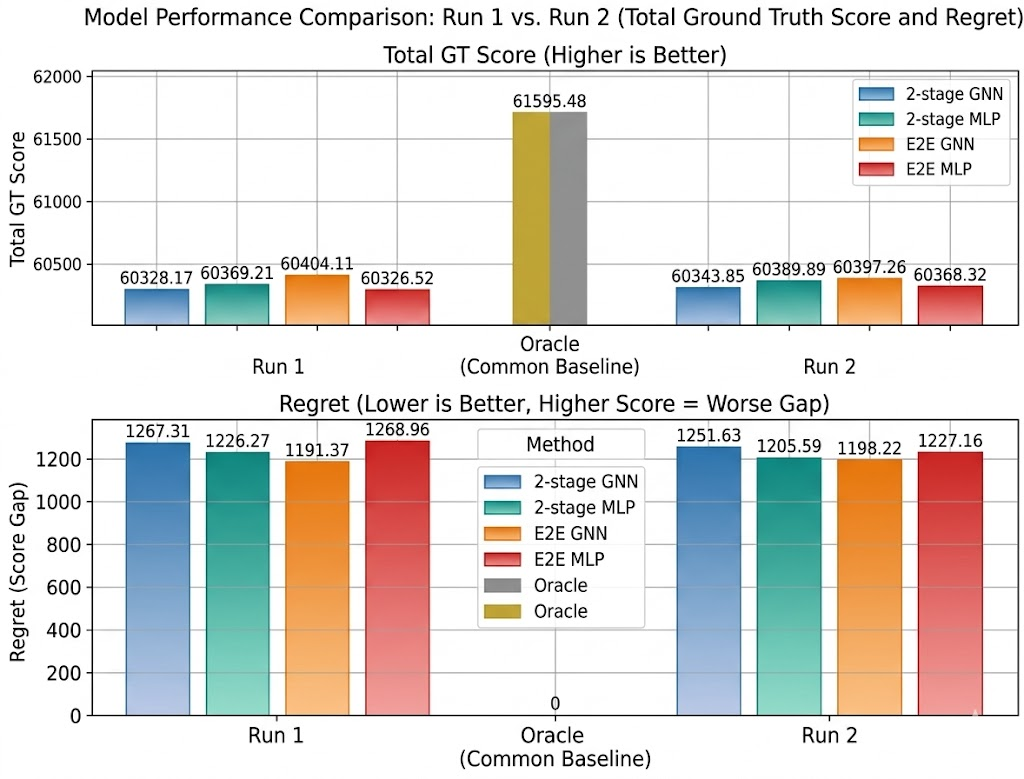
\includegraphics[width=0.88\textwidth]{Results.jpg}
\caption{Visual summary of the main results}
\label{fig:main-results-bars}
\end{figure}

The main conclusions from this comparison are as follows. First, the oracle benchmark remains clearly above all learned methods, confirming that there is still a substantial gap between learned edge scoring and the best achievable exchange plans under the same optimization model. Second, the end-to-end GNN consistently improves over the corresponding two-stage GNN baseline across both runs, with modest but repeatable gains in total ground-truth score. This suggests that decision-focused learning can provide useful downstream improvements when combined with a graph-aware predictor. Third, the MLP-based end-to-end models do not outperform their corresponding two-stage MLP baselines, indicating that the benefit of decision-focused learning is architecture-dependent in the current setup. Finally, the learned methods often perform more transplants than the oracle while still achieving lower total ground-truth score, highlighting that maximizing transplant count and maximizing total exchange quality are not equivalent objectives in this setting.

\subsection{A Sanity Check on the Current Synthetic Labels}
The experiments above compare different learning-and-optimization pipelines under a common downstream KEP solver. However, an additional diagnostic on the current synthetic label construction reveals an important limitation of the present benchmark: our labels are strongly aligned with local edge-level information, which makes the benchmark naturally favourable to two-stage supervised learning.

In the current data-processing pipeline, each edge label is generated from edge-local clinical proxies. In particular, the synthetic ground-truth edge score is computed from a success-probability term, a QALY-style term, and a small multiplicative perturbation:
\[
w_{\mathrm{true},e}
\approx p_{\mathrm{succ},e}\cdot \mathrm{QALY}_e \cdot (1+\epsilon_e),
\]
where both \(p_{\mathrm{succ},e}\) and \(\mathrm{QALY}_e\) are themselves functions of donor-recipient information already available at the edge level, most notably the utility score, recipient cPRA, and donor age. Moreover, the raw edge utility is included directly in the model input. Hence, the stage-1 learning problem is already very close to directly regressing the quantity used by the stage-2 optimizer.

To quantify this effect, we performed two simple sanity-check baselines on the same processed batch (\texttt{2026-03-31\_140543}) and on the same common train/validation/test split used by the main experiments. The first baseline regresses \(w_{\mathrm{true}}\) using only the single scalar edge utility. The second baseline uses a linear ridge regressor over purely local edge features, namely source-node features, target-node features, and the scalar edge utility, but still no graph message passing and no end-to-end optimization. Table~\ref{tab:label-sanity-a} reports the resulting edge-level diagnostics.

\begin{table}[t]
\centering
\small
\setlength{\tabcolsep}{5pt}
\caption{Edge-level sanity checks for the current synthetic labels on batch \texttt{2026-03-31\_140543}. Correlation is the Pearson correlation between edge utility and the synthetic ground-truth label. The ``edge-only linear'' baseline uses only local donor-recipient and edge features, with no graph topology.}
\label{tab:label-sanity-a}
\begin{tabular}{@{}lrrr@{}}
\toprule
\textbf{Quantity} & \textbf{Train} & \textbf{Val} & \textbf{Test} \\
\midrule
\( \mathrm{corr}(\mathrm{utility}, w_{\mathrm{true}}) \) & 0.7738 & 0.7762 & 0.7663 \\
Utility-only MSE & 9.6140 & 9.4672 & 10.2839 \\
Edge-only linear MSE & 3.3251 & 3.2729 & 3.5897 \\
\bottomrule
\end{tabular}
\end{table}

The utility--label correlation is already high (\(\approx 0.77\)) on every split. More importantly, a purely local linear predictor---without any graph-aware representation learning---already achieves a test MSE of 3.59, which is surprisingly competitive relative to the learned GNN and MLP models used in the main experiments.

We next pushed these baselines through the same downstream hybrid KEP optimizer. Table~\ref{tab:label-sanity-b} compares their final decision quality against the main learned methods on the common 10-graph test split. The key observation is that even the utility-only baseline, which sees only one scalar feature per edge, is already close to the graph-aware end-to-end methods; and the edge-only linear baseline is competitive with, or better than, several DFL variants.

\begin{table}[t]
\centering
\small
\setlength{\tabcolsep}{4pt}
\caption{Downstream decision quality on the common 10-graph test split of batch \texttt{2026-03-31\_140543}. ``Achieved'' denotes the average ground-truth objective value obtained by the selected exchange plan, and ``Regret'' is measured against the oracle. The last two rows are the sanity-check baselines described in the text.}
\label{tab:label-sanity-b}
\begin{tabular}{@{}lrr@{}}
\toprule
\textbf{Method} & \textbf{Avg Achieved} & \textbf{Avg Regret} \\
\midrule
2-stage GNN & 308.1811 & 9.1698 \\
2-stage MLP & 310.2835 & 7.0675 \\
FY-DFL GNN & 307.0828 & 10.2681 \\
FY-DFL MLP & 309.8360 & 7.5149 \\
SPO+ GNN & 307.4284 & 9.9225 \\
SPO+ MLP & 309.9184 & 7.4325 \\
SPO+ + MSE anchor GNN & 307.6322 & 9.7188 \\
SPO+ + MSE anchor MLP & 310.2409 & 7.1101 \\
\midrule
Edge-only linear baseline & 307.6529 & 9.6981 \\
Utility-only baseline & 306.4726 & 10.8783 \\
\bottomrule
\end{tabular}
\end{table}

These numbers strongly suggest that the current synthetic label design does not yet provide a demanding test bed for decision-focused learning. The benchmark largely rewards accurate local edge regression, because the synthetic label is generated from edge-level quantities that are already exposed, or very nearly exposed, to the predictive model. As a result, a two-stage pipeline is naturally advantaged: once edge scores are regressed well, the subsequent optimization problem is already close to the true objective.

Therefore, while the current experiments remain useful for validating implementations and for comparing solver formulations under a controlled synthetic setting, they should not be over-interpreted as evidence about the intrinsic value of decision-focused learning for real KEP objective design. In future work, the data-generation process should be revised so that final exchange quality depends less directly on a nearly observable edge-local score and more on medically meaningful program-level considerations, such as failure-aware utility, priority for hard-to-match recipients, or dynamic opportunity cost. Only under such a setting can we fairly test whether end-to-end KEP learning genuinely outperforms a strong two-stage baseline.

\subsection{A Solver-Time Comparison Across Formulations}
Besides solution quality, the optimization formulation also changes the practical computational cost of the pipeline. To isolate this effect from learning dynamics, we followed the timing procedure in \texttt{formulations/README.md} and compared only the stage-2 solver entry points. Concretely, we ran \texttt{formulations/cf/stage2\_solver.py}, \texttt{formulations/hybrid/stage2\_solver.py}, and \texttt{formulations/pief/stage2\_solver.py} with the same processed batch (\texttt{2026-03-31\_140543}), the same warm-start MLP checkpoint, and the same solver limits (\texttt{max\_cycle}=3, \texttt{max\_chain}=4). In all three cases, the solver processed the same 50 graphs and wrote a complete set of solutions. We measured runtime with \texttt{/usr/bin/time -p}, so the key quantity is the wall-clock time reported in the \texttt{real} field.

Table~\ref{tab:solver-speed} shows a clear formulation-level efficiency gap. The hybrid formulation is the fastest in this experiment, requiring only 3.64 seconds for the full batch, compared with 11.05 seconds for the pure candidate-formulation baseline. The dual-PIEF formulation is also substantially faster than CF, but remains slower than the hybrid design. Put differently, under the same input weights and the same KEP instances, the hybrid solver is about \(3.04\times\) faster than CF, while PIEF is about \(2.28\times\) faster than CF.

\begin{table}[t]
\centering
\small
\setlength{\tabcolsep}{5pt}
\caption{Solver-only runtime comparison across formulations on batch \texttt{2026-03-31\_140543}, using the exact stage-2 timing setup from \texttt{formulations/README.md}. Lower is better. Speedup is computed relative to CF using wall-clock time.}
\label{tab:solver-speed}
\begin{tabular}{@{}lrrrr@{}}
\toprule
\textbf{Formulation} & \textbf{Real (s)} & \textbf{User (s)} & \textbf{Sys (s)} & \textbf{Speedup vs CF} \\
\midrule
CF (\texttt{CF-CYCLE + CF-CHAIN}) & 11.05 & 17.17 & 1.02 & \(1.00\times\) \\
Hybrid (\texttt{CF-CYCLE + PIEF-CHAIN}) & 3.64 & 10.51 & 0.27 & \(3.04\times\) \\
PIEF (\texttt{PIEF-CYCLE + PIEF-CHAIN}) & 4.85 & 12.66 & 0.39 & \(2.28\times\) \\
\bottomrule
\end{tabular}
\end{table}

This finding matters methodologically. It shows that formulation choice is not merely an implementation detail hidden behind a common black-box solver interface; it directly changes the runtime profile of KEP optimization. In the present setup, the hybrid formulation delivers the best efficiency among the three tested alternatives, suggesting that formulation engineering can produce large practical gains even before considering any changes in predictive accuracy or learning objective.

\bibliographystyle{plainnat}
\bibliography{ref}
\end{document}
